\chapter{Conclusions and future lines}\label{ch:conclusions}
Taking into consideration the results presented in Chapter~\ref{ch:experiments}, we are now able to draw conclusions and discuss whether the goals established in Section~\ref{sec:goals} can be considered fulfilled or not. For ease of reading, we will articulate our conclusions following the structure of the aforementioned goals, pointing out our main contributions and the challenges that we have found along the way. Finally, we will conclude our report looking ahead for potential improvements of the system we have designed, as well as proposing new applications and related research topics that are yet to be explored.

\section{Main conclusions}
\subsubsection{Quantitative evaluation of 2D human pose estimation methods}
The proposed method relies on an accurate 2D human pose estimation from which to infer the corresponding three-dimensional locations of the joints. Taking this requirement into consideration, we needed a robust 2D pose estimator that could serve as a backbone for the system we were designing. Here are our conclusions in that regard:

\begin{itemize}
    \item A thorough review of the literature has been done in order to found those solutions that better fit our requirements. Human pose estimation is a very active area within the field of computer vision, and so there is large number of available publications that we have explored and analyzed.
    \item After this first stage of exploration, we have selected three \gls{sota} methods: \emph{Convolutional Pose Machines}~\cite{Wei2016-rb}, \emph{Stacked Hourglass}~\cite{Newell2016-cy} and \emph{Chained Predictions}~\cite{Gkioxari2016-ix}. All of them share some characteristics that made them appropriate for our purposes: they are relevant works in the field, their code is publicly available and they claim to reach a good trade-off between performance and computational cost.
    \item In order to validate the results provided in their respective articles, we have performed an exhaustive quantitative evaluation and comparison of the three methods mentioned above. This evaluation has been carried out using an international publicly available dataset (\gls{bmhad}) that contains more than 1300 scenes, which shows different subjects performing a variety of actions. Overall, \emph{Convolutional Pose Machines} have achieved better results than \emph{Stacked Hourglass} and \emph{Chained Predictions}, and so it is our go-to estimator for the designed system. Besides that, the difference between \emph{Convolutional Pose Machines} and the other methods is specially significant for the most challenging scenes in the dataset.
    \item After validating their performance, the three tested estimators have been successfully integrated in our pipeline. Looking back at the designed system for the real-time demo in Section~\ref{sec:demo}, the user can choose between any of these methods for 2D estimation before launching the application by simply updating a configuration file.
\end{itemize}

We can conclude that suitable solutions for 2D pose estimation have been researched, tested and, finally, integrated in our system, accomplishing the goal established in Section~\ref{sec:goals}. It is important to note that this field of research is evolving at an impressive pace, and so our method may fall short in comparison with most recent works if this core component of our application does not get regularly updated. 

\subsubsection{Development of a pipeline for augmenting 2D to 3D pose estimations}
The main focus of this project has been the development of a system that, taking as input an RGBD video sequence, estimates 3D human poses keeping a fair trade-off between accuracy and computational cost. We have already talked about the first step in that process, which is estimating the 2D joint locations in the RGB image. In order to take these 2D estimations to 3D using the information provided by the depth image, a lightweight algorithm was required. Here are our conclusions in that regard:

\begin{itemize}
    \item In order to understand what kind of processing our algorithm needed to perform on the input data, we have explored the main issues that arise when trying to infer 3D estimations from the 2D locations and the depth image without any intermediate step.
    \item After exploring these results, we have looked for solutions that were both effective and lightweight. Taking these considerations into account, we have developed a very straight-forward algorithm that allows us to estimate the 3D poses with respectable accuracy in real-time. Our approach pre-processes the input depth map and 2D coordinates by means of a \emph{Gaussian} blur and a minima filter, reprojects the result to 3D, rejects outliers and smooths the resulting estimations using a \emph{Kalman} filter for each joint.
    \item We have implemented our system in \emph{Python} using common libraries for image and data processing. Our source code has been made publicly available and it is hosted in a \emph{GitHub} repository~\footnote{\url{https://github.com/RoboticsLabURJC/2017-tfm-david-pascual}}.
\end{itemize}

In summary, we have developed an agile algorithm that is able to yield 3D human pose estimations given its corresponding 2D joint locations and a depth map. Our pipeline takes a video sequence from an RGBD camera and, making use of the 2D estimation methods previously discussed, returns three-dimensional poses for the subject in the scene in real-time. In that sense, we have fulfilled the goal established in Section~\ref{sec:goals}. Nonetheless, further improvements can be explored, \eg our mechanisms for filtering the estimations could be more adaptive and some processes performed independently for each joint could be parallelized.

\subsubsection{Quantitative evaluation and comparison of our proposed method}
In order to experimentally validate the conclusions reached in the paragraph above, an exhaustive quantitative evaluation was needed. Furthermore, it is important to put our work in context and check how the achieved results compare with the \gls{sota}. Again, one major requirement of this project is keeping the computational cost as low as possible, and so this is a topic that also required analysis. Here are our conclusions regarding the quantitative evaluation of our work:

\begin{itemize}
    \item A comparison between the proposed method and a simple baseline has been performed. For that purpose, we define as baseline the direct inference of the 3D coordinates given the 2D locations and the depth map, without further processing. Using a subset of the \gls{bmhad} dataset (132 scenes) and using \gls{mpjpe} as figure of merit, we have validated that the inclusion of the proposed method improves significantly the final estimations.
    \item Further analysis of this comparison has demonstrated how our processing is specially beneficial when 2D estimations are slightly misplaced, as this can result in huge differences in 3D. It is worth mentioning that, if the 2D location is accurate and there is no self-occlusions or other kind of interference, we find no significant difference in the results yielded by our method and the baseline.
    \item After assessing the improvements introduced with respect to the baseline, we have analyzed how the measured error correlates with the dimensions of the three-dimensional space. We have discovered that most of the committed error comes from the \(Z\) dimension, \ie  the distance between the camera and the subject. As mentioned before, slight deviations in the 2D estimation might also cause great differences in 3D.
    \item A comparison with a \gls{sota} method has been performed. A large portion of the amount of effort put into this work has been dedicated to this comparison. We have thoroughly evaluated our algorithm against the solution proposed by Zimmermann \etal\cite{Zimmermann2018-sn} in order to assess whether the designed system is good enough to justify its application in real scenarios. For that purpose, we have used the \gls{bmhad} dataset in its entirety. \gls{pckh} and \gls{mpjpe} have been employed to measure performance. All of the results have been presented grouped by joints and by actions and action types.
    \item This experimental comparison has allowed to reach several relevant conclusions. First of all, our method is very competitive when compared with the \gls{sota}, but we cannot outperform it. Surprisingly, our method performed better for some of the most heavily occluded scenes and yielded a very respectable \gls{pckh}. We attribute these results mainly to our explicit outlier rejection mechanism, which avoids committing huge errors even if the scene is very challenging. However, under normal circumstances, Zimmermann's algorithm deals better with self-occlusions as their model implicitly learns priors about how a human body is supposed to appear.
    \item Last but not least, we have analyzed the computational burden associated with our system. We demonstrate that our method is significantly faster than Zimmermann's. Our module for 3D estimation alone takes about 10ms per frame, fulfilling the major requirement of keeping the computation costs low. These small times per frame means that the final estimation time are highly dependant on the 2D estimator used. 
\end{itemize}

Taking into consideration all of the conclusions drawn above, we can consider the goal defined in Section~\ref{sec:goals} accomplished. We have carried out a very exhaustive evaluation of our method against a baseline and a \gls{sota} method, both in terms of accuracy and computational cost. With these results, our system seems to fulfill the major requirements we impose for it to work as component in robotics applications, reaching a reasonable trade-off between its agility and performance. 

\subsubsection{Qualitative evaluation of our proposed method: real-time demo}
The resulting product of all of the aforementioned research in the previous section is a real-time demo which has allowed us to validate how our system might work in a real environment. This is a major milestone as it puts the theoretical knowledge acquired during this project into practice. Here are our conclusions in that regard:

\begin{itemize}
    \item A working real-time application for 3D human pose estimation has been developed. This application uses an \emph{off-the-shelf} computer and a commercial RGBD sensor, and integrates the method described in Chapter~\ref{ch:proposed_method} within an environment built in \emph{Python} that handles communication with the sensor, estimation and visualization in a threaded manner. Code and instructions for running the application are publicly available in \emph{GitHub}~\footnote{\url{https://github.com/RoboticsLabURJC/2017-tfm-david-pascual}}.
    \item A demo has been carried out to assess the feasibility of our system. The results have been recorded and the resulting video is publicly available~\footnote{\url{https://www.youtube.com/watch?v=W3XirsadmNg}}. For this demonstration, we built a very simple setup comprised of a common PC and an \emph{Asus XTION PRO LIVE} RGBD camera. A subject placed in front of the camera interacts with the application in real-time successfully.
    \item During the recording of this demo, we also documented failure cases, being the most significant self-occlusions and excessive proximity to the camera. These results match the conclusions drawn during the quantitative evaluation of our method.
\end{itemize}

Recalling the requirements imposed for an algorithm to be embedded in a robotic system, we pointed out that it must work in real-time in an \emph{off-the-shelf} computer, with a regular RGBD camera and independently of the point of view. Taking these into account, we can consider our major goals fulfilled as demonstrated by our real-time demo. The weakest point of the proposed method might be the point of view of the camera, not because of the position of the camera itself, but due to the possibility of increasing the number of occlusions, which our algorithm struggles to handle. Nonetheless, we have reached our major milestone of building an application that runs in real-time and estimates 3D human poses with an average error of 144mm, which is a very reasonable trade-off that would justify its inclusion as a core component in robotics applications.

\section{Future work}
Thanks to the knowledge acquired during the development of this project and given that we have built a stable infrastructure for the task of 3D pose estimation, a great amount of potential applications and improvements are on the table. In this section, we will discuss some of them, leaving an open door for further research on the topic.

\begin{itemize}
    \item Probably the most evident improvement we can make to our pipeline is regularly updating the model used for estimating the 2D locations of the joints. This is possibly a never-ending task, as new works claiming to achieve better results arise every year. However, it seems like the magnitude of these incremental improvements is starting to plateau, as it can be seen in Figure~\ref{fig:mpii_results}. Nonetheless, it is worth reviewing the literature regularly and updating our system consequently.
    
    \begin{figure}[h]
        \centering
        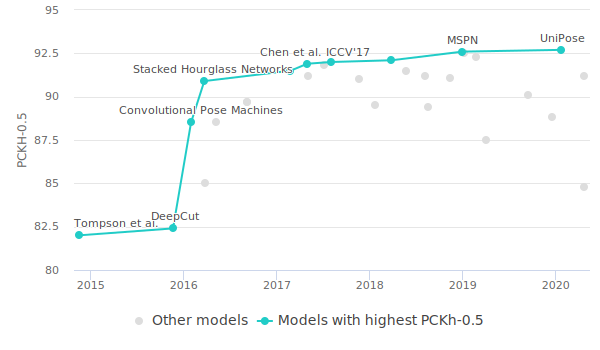
\includegraphics[width=\textwidth]{figures/chart.png}
        \caption{In this graph, publicly available methods for 2D pose estimation presented in the last years evaluated against the MPII dataset are shown (source \cite{papers_with_code}). Note that the methods we tested (CPMs and SH) were a major breakthrough in the field. Since then, new methods have slightly outperformed them, but the improvements are starting to plateau.}
        \label{fig:mpii_results}
    \end{figure}

    \item Another possible improvement regarding 2D estimation is further reducing the inference time. As accuracy starts to peak, efficiency should become one of the main priorities for new works in the field. For instance, in the object detection field very efficient architectures have been explicitly developed for being embedded in systems with scarce resources~\cite{sandler2018mobilenetv2}. Such is the case of the very recently introduced \emph{EfficientPose}~\cite{groos2020efficientpose}, which claims to be 20 times more computationally efficient than \emph{OpenPose}~\cite{cao2018openpose} while outperforming it. Including this kind of new approaches could be a major improvement for our application which could then be integrated in cheaper devices.
    \item Multi-person pose estimation has been left unexplored in this project, but it could be an important requirement depending on the particular application. To that extent, we presented some works focusing on multi-person scenarios in Chapter~\ref{ch:related_work}, being the most prominent the one proposed by Cao \etal\cite{cao2018openpose}, which builds upon \glspl{cpm} and is the core of the \emph{OpenPose} suite. Evaluating how this method performs and analyzing whether its computational cost is low enough for robotics applications might be a natural extension of our work.
    \item Yet another improvement that could be considered for our current pipeline is including stronger hints of how a human body should look like to further improve our results. In other words, introducing priors for the human poses could allow us to manage complex scenearios with self-occlusions and so on. \gls{dl} models such as the one proposed by Zimmermann \etal\cite{Zimmermann2018-sn} are too computationally intensive for our approach, but we could consider fitting simpler human body models or researching more lightweight \gls{dl} architectures for that purpose.
    \item Regarding the evaluation stage of our project, it would be desirable to include more natural \textit{in-the-wild} scenes with more points of view to further validate how our method and \gls{sota} solutions perform in the real world. In that sense, finding or building a dataset containing RGBD data and accurate labels for the 3D poses would be needed.
    \item One possibility that we have not yet mentioned is using our approach for getting 3D coordinates from 2D pose estimation data from other articulated objects or subjects that might not necessarily be humans, after updating our outlier rejection criteria. For instance, it could be used for estimating hand poses~\cite{Chang2018} or poses in animals~\cite{kearney2020rgbd}, which could open the doors for very interesting applications. In Figure~\ref{fig:examples_articulated}, examples of such approaches can be seen.
    
    \begin{figure}[h]\centering
        \begin{subfigure}{0.49\textwidth}\centering
            \includegraphics[height=5.75cm]{figures/hand_pose.png} 
            \caption{3D hand pose estimation~\cite{Chang2018}}
            \label{subfig:hand_pose}
        \end{subfigure}
        \begin{subfigure}{0.49\textwidth}\centering
            \includegraphics[height=5.75cm]{figures/animal_pose.png}
            \caption{3D dog pose estimation~\cite{kearney2020rgbd}}
            \label{subfig:animal_pose}
        \end{subfigure}
        \caption{Our algorithm could be adapted for estimating 3D poses for other articulated objects or subjects, such as (a) hands or (b) animals.}
        \label{fig:examples_articulated}
    \end{figure}

    \item Finally, the most obvious follow-up for our work is integrating our approach, as demonstrated in Section~\ref{sec:demo}, in a real robotic application. 3D human pose estimation can be included as a core component for solving tasks such as fall detection or action recognition of any kind, which is very useful information for any human-robot interaction. In that sense, our algorithm could be applied in fields such as assistive robotics, for which human-awareness is a major requirement.
\end{itemize}

In summary, our work can be considered in itself the basis from which bigger embedded applications can be built upon. Further improvements and evaluations may be considered in order to make our method more effective and stable, and more robust in challenging scenarios. Besides these improvements, it can be extended for estimating poses in multi-person scenarios or supporting other articulated objects. Integrating our system in a real-world robotic application, with or without these extensions and improvements, is the next major milestone for this project.
